% !TeX spellcheck = de_CH_frami

Die Analyse und sp\"atere Synthese von Funktionen ist ein wichtiges 
mathematisches Instrument, dass bei vielen Problemen eingesetzt wird. Die 
Fourier- und die Wavelettheorie geh\"oren dabei zu den prominentesten Methoden.

F\"ur viele Probleme lassen sich nur schwer kontinuierliche Funktionen finden, 
die den vorhanden Sachverhalt genau wiedergeben. In der heutigen digitalen Zeit 
liegen die Daten meist nur in diskreter Form vor und m\"ussen beziehungsweise 
k\"onnen ur so weiterverarbeitet werden.

F\"ur die Analyse und Synthese brauchen wir jeweils Basisfunktionen mit dessen 
wir die Vor- und sp\"atere R\"ucktransformation durchf\"uhren k\"onnen.
Funktionen mit eindimensionale Definitionsbereich $f: \mathbb{R} \rightarrow 
\mathbb{R}$ stellen die Exponentialfunktion $e^{i2\pi\omega x}$ eine m\"ogliche 
Basis dar, diese wird meist in der klassischen Fouriertheorie verwendet. Im 
zweidimensionalen Fall $f: \mathbb{R}^2 \rightarrow \mathbb{R}$ wie 
beispielsweise einem Bild, wird oft einfach jeweils eine eindimensionale 
Transformation f\"ur jeweils eine Dimension vorgenommen, man erh\"alt dann 
Basisfunktionen der Form $e^{i2\pi(ux+vy)}$. Mit drei Dimensionen $f: 
\mathbb{R}^3 \rightarrow \mathbb{R}$ wie zum Beispiel Kugeloberfl\"achen, gibt 
es die Kugelfunktionen $Y^m_l$, welche eine Basis darstellen.

\begin{figure}
    \centering
    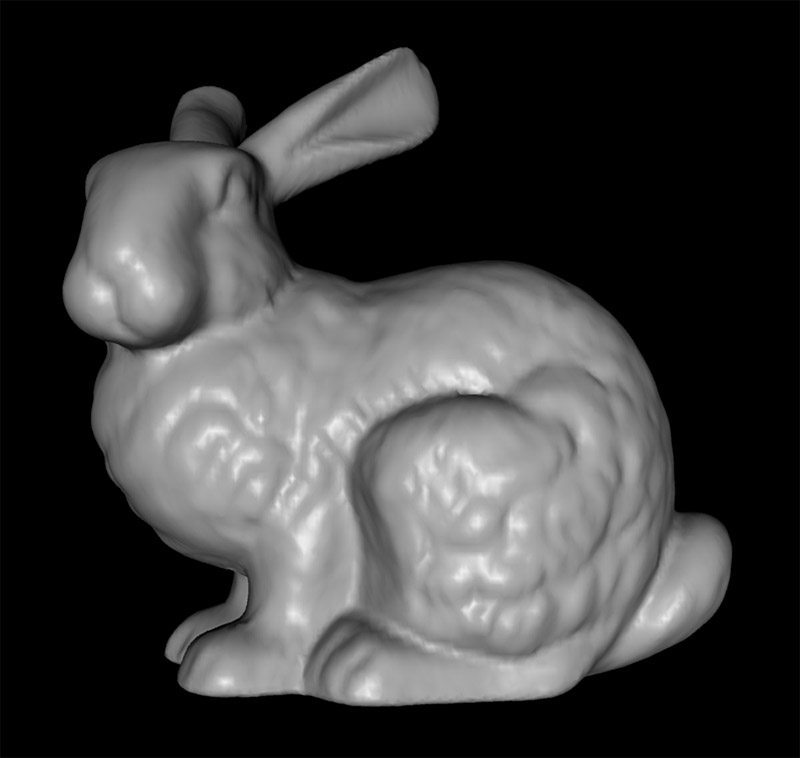
\includegraphics[
    scale=0.3
    ]{papers/sgwt/images/bunny-scanalyze-sh.jpg}
    \caption{Der Standford Bunny~\cite{noauthor_stanford_nodate} ist eines der 
    bekanntesten Testmodelle, wenn 
    es um Computergraphiken geht.
        \label{fig:sgwt:intro:bunny}}
\end{figure}


Was ist nun aber mit Funktionen die nicht auf einfachen K\"orperoberfl\"achen 
liegen? Zum Beispiel Funktionen auf der Oberfl\"ache des ber\"uhmten 
``Standford Bunnys''~\cite{noauthor_stanford_nodate}, zu sehen in 
\cref{fig:sgwt:intro:bunny}, welches oft als Testmodell f\"ur Computergraphiken 
eingesetzt wird. Oder bei Modellen deren Unterliegende Oberfl\"ache keine, 
oder nur nebens\"achliche, Rolle spielt, wie bei Routernetzerwerken, 
Strassennetzen oder ganz generell wenn wir nur einen Graphen haben?

In diesem Kapitel wollen wir deshalb eine Theorie entwickeln, wie 
wir die bereits bekannte Fourier- und Wavelettheorie auch auf Graphen anwenden 
k\"onnen, bei dem die Funktion auf seine Knoten abgebildet wird. Diese Theorie 
ist bekannt als Spectral Graph Wavelet Transform oder kurz SGWT -- nicht zu 
verwechseln mit der Second Generation Wavelet 
Transform~\cite{noauthor_second-generation_2018}, deren K\"urzel ebenfalls SGWT 
lautet -- die erstmals 2009 in ``Wavelets on Graphs via Spectral Graph 
Theory''~\cite{hammond_wavelets_2009} vorgestellt wurde. Wir startet mit 
einigen Grundlagen \"uber Graphen in~\cref{sec:sgwt:graphs}, gehen dann zum 
Laplace Operator und Matrix in~\cref{sec:sgwt:laplace} 
und landen schliesslich bei der Spektral Graph Wavelte Transformation 
in~\cref{sec:sgwt:spectralanalysis}.
